\documentclass[slidestop, compress, mathserif]{beamer}

\usepackage[style=authoryear-comp, sorting=nyt, maxcitenames=2, backend=biber]{biblatex}
\renewbibmacro{in:}{}
\renewcommand\bibfont{\small}
\addbibresource{ref.bib}

\usepackage{amsmath, amssymb, mathrsfs}
\usepackage{color, graphicx}

\usepackage{setspace, listings}
\usepackage{sidecap}

\usetheme{Madrid}
\usecolortheme{default}
\linespread{1.2}



\sidecaptionvpos{figure}{c}
\usepackage[textfont=small]{caption}
\setbeamertemplate{caption}[numbered]
\captionsetup{font=scriptsize, labelfont=scriptsize, labelformat=simple}

\setbeamertemplate{footline}
{
  \leavevmode%
  \hbox{%
  \begin{beamercolorbox}[wd=1.0\paperwidth,ht=2.25ex,dp=1ex]{author in head/foot}\usebeamerfont{author in head/foot}
    \hspace*{3ex}
    \inserttitle
    \hfill
    % \insertshortauthor
    % \insertfirstauthor
    Gun Woo Park 
    \hspace{1em}\insertshortdate
    \hspace{1em}\insertframenumber/\inserttotalframenumber
    \hspace*{3ex}
  \end{beamercolorbox}%
}%
  \vskip0pt%
}

\title{MSD Analysis for Data RT=1 (ICR Abstract)}
% \institute{DICMaPI, University of Naples Federico II}
% \author{Gun Woo Park, Giovanni Ianniruberto, and Giuseppe Marrucci}
\author{Gun Woo Park}
% \date{13 APR 2016}


% it's for headline
\setbeamertemplate{headline}{%
  % \leavemode%
  \hbox{%
    % \begin{beamercolorbox}[wd=\paperwidth,ht=2.5ex,dp=1.125ex]{palette quaternary}%
    \begin{beamercolorbox}[wd=\paperwidth,ht=2.5ex,dp=1.125ex]{section in head/foot}%
      \insertsectionnavigationhorizontal{\paperwidth}{}{\hskip0pt plus1filll}
    \end{beamercolorbox}%
    }
}

\begin{document}

\begin{frame}
  \maketitle
\end{frame}

\begin{frame}
  \frametitle{MSD comparison}
  \begin{figure}
    \centering
    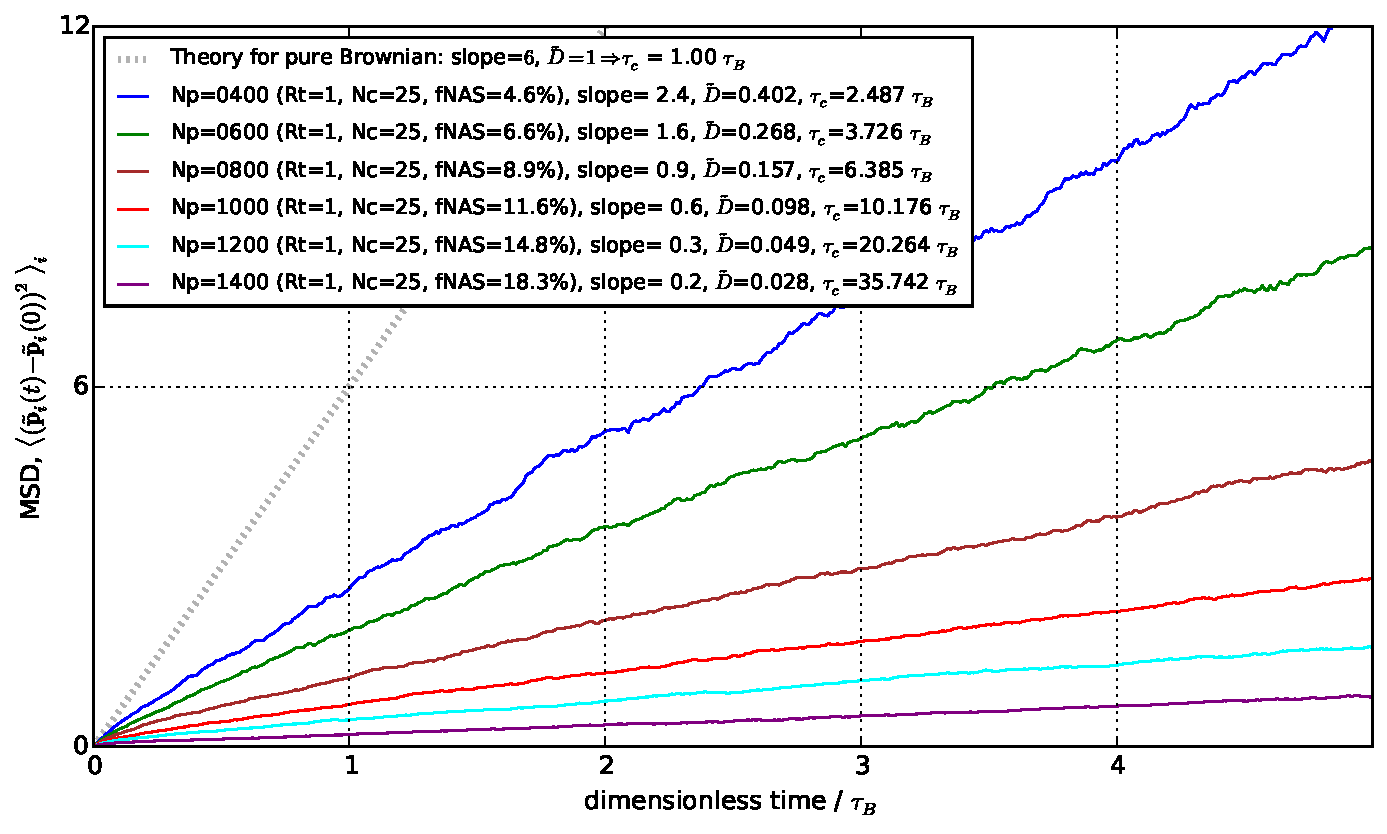
\includegraphics[width=\textwidth]{../diffusion_map.pdf}
  \end{figure}
\end{frame}

\begin{frame}
  \frametitle{Diffusion Coefficient}
  \begin{figure}
    \centering
    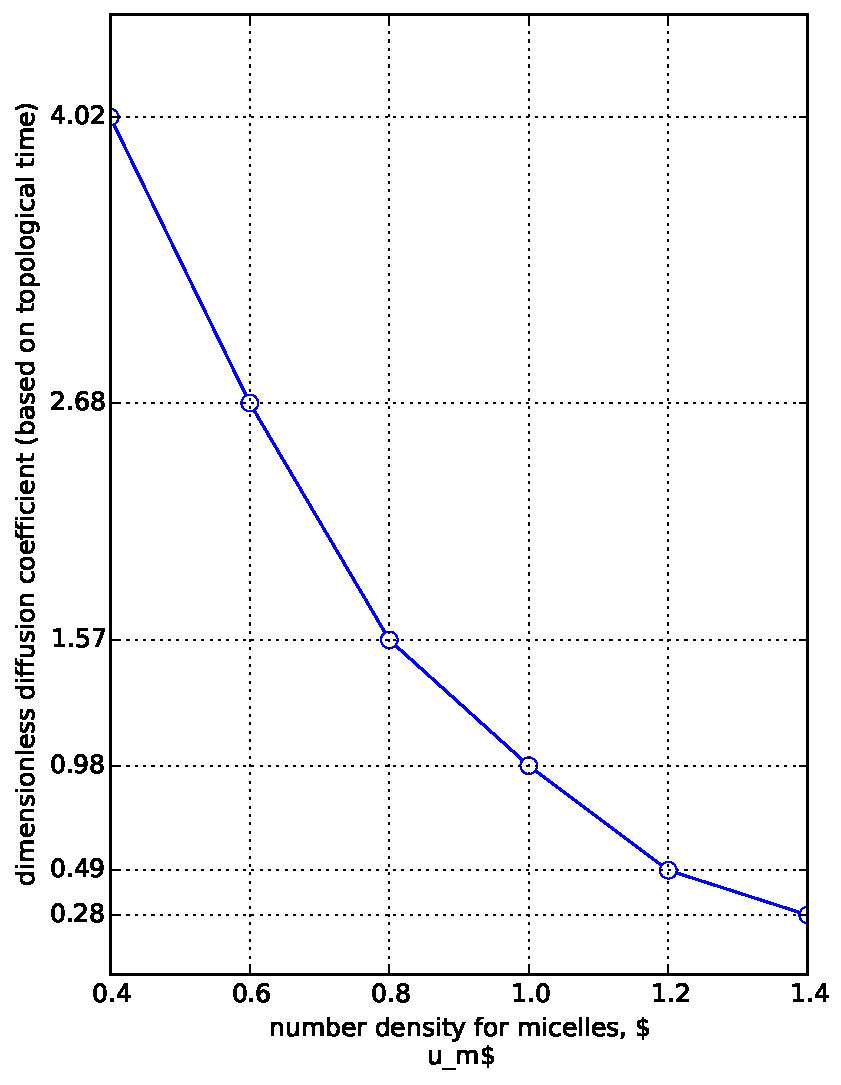
\includegraphics[width=0.45\textwidth]{../diffusion_coefficient.pdf}
    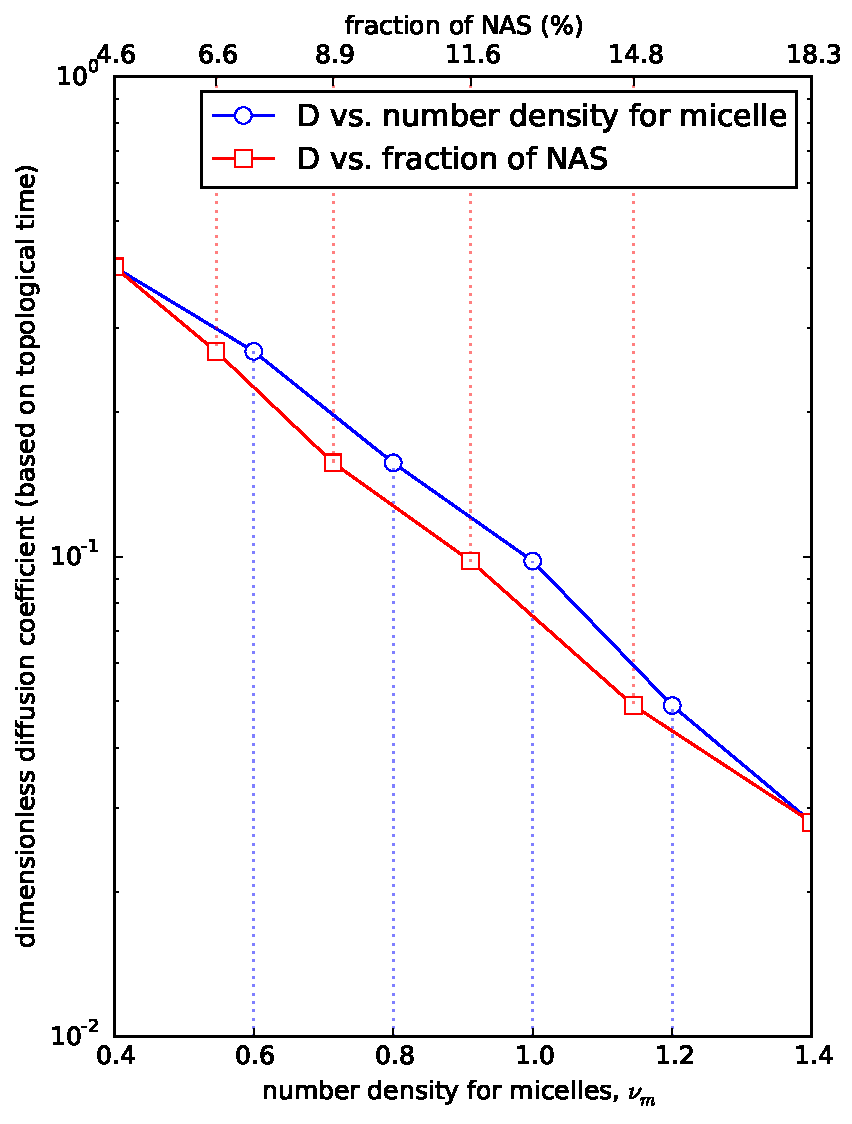
\includegraphics[width=0.45\textwidth]{../diffusion_coefficient_semilogy.pdf}
  \end{figure}
\end{frame}

\begin{frame}
  \frametitle{Diffusion Time: $\tau_c = \frac{R_0^2}{D} \Rightarrow \tilde{\tau_c} = \frac{1}{\tilde{D}}$}
  \begin{figure}
    \centering
    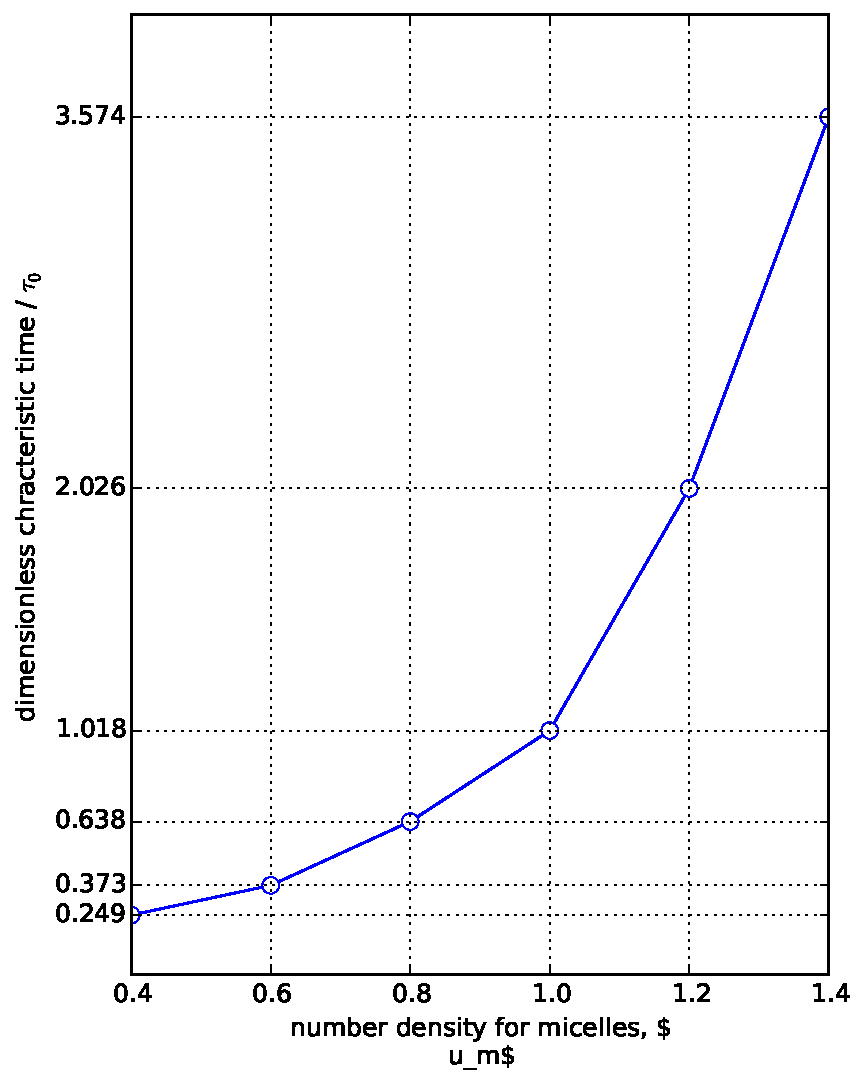
\includegraphics[width=0.45\textwidth]{../characteristic_time.pdf}
    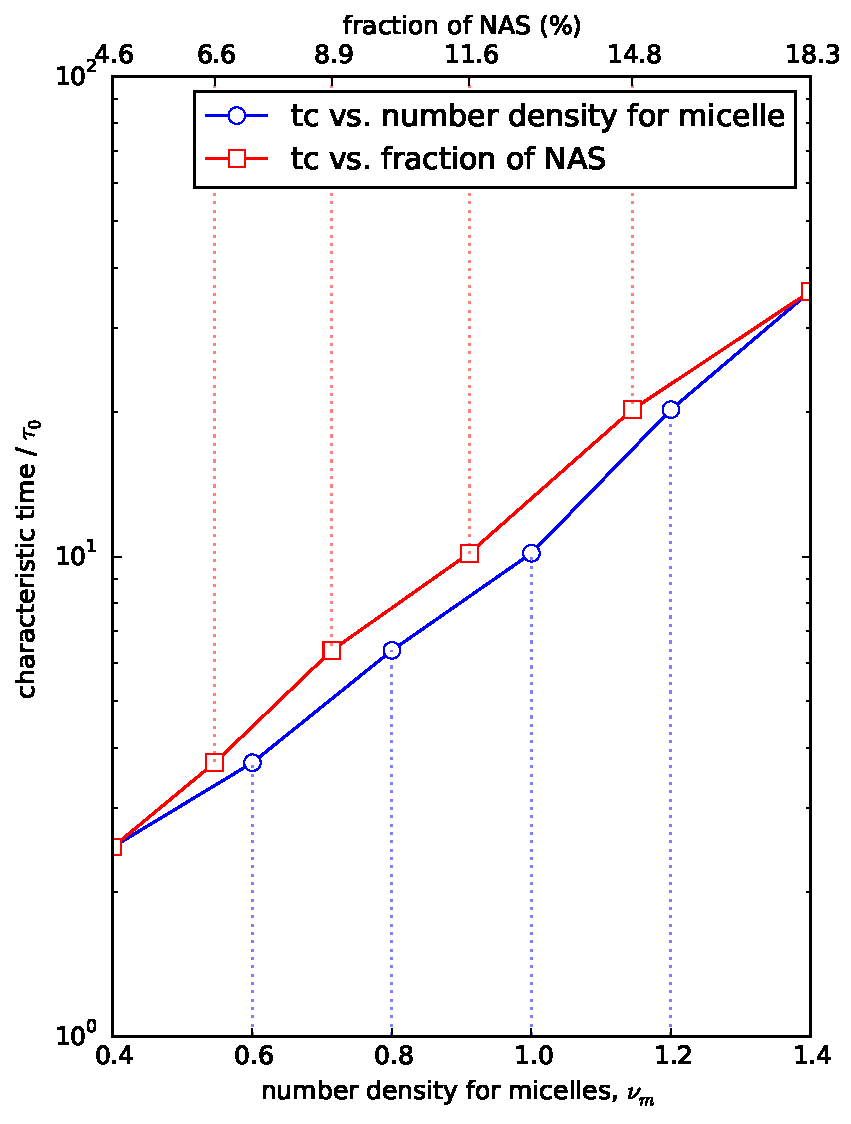
\includegraphics[width=0.45\textwidth]{../diffusion_time_semilogy.pdf}
  \end{figure}
\end{frame}
\begin{frame}
  \frametitle{Scaling Law for Diffusion Time}
  \begin{figure}
    \centering
    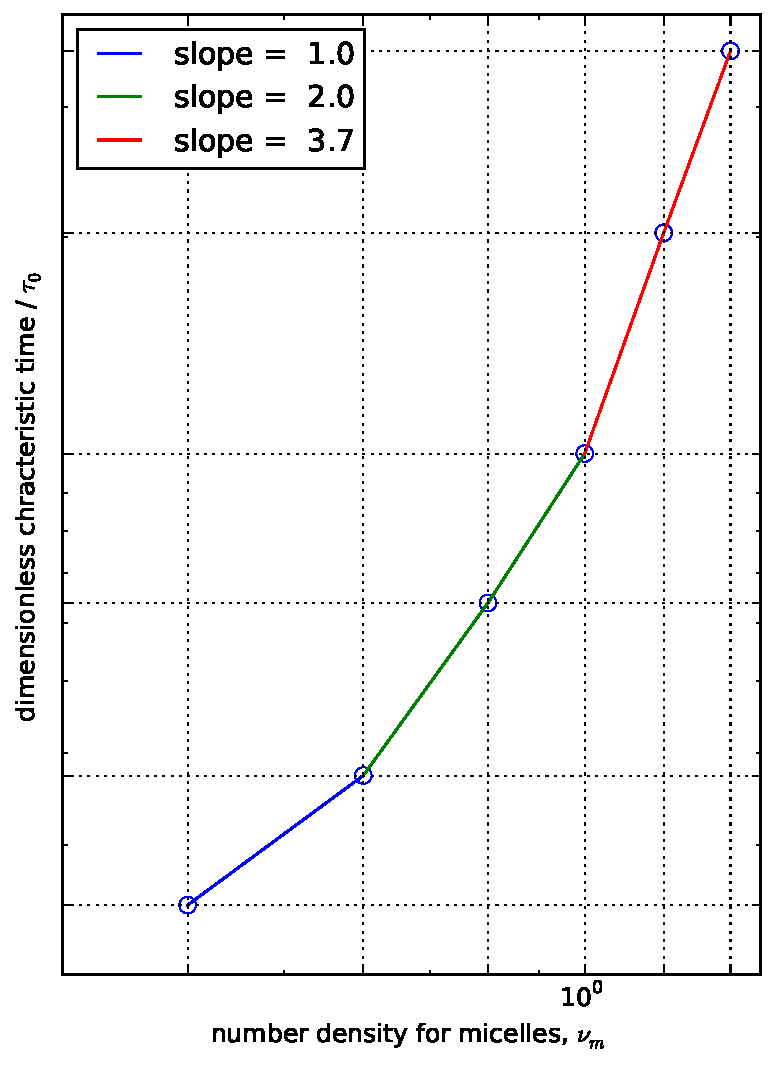
\includegraphics[width=0.45\textwidth]{../characteristic_time_loglog.pdf}
  \end{figure}
\end{frame}

\end{document}
% \section{Overview}
% \begin{frame}
%   \frametitle{Linear Viscoelasticity for HEUR Solution}
%   \begin{figure}
%     \centering
%     \includegraphics[width=0.4\textwidth]{figures/dynamic_moduli_Suzuki_2012.png}
%     \includegraphics[width=0.3\textwidth]{figures/scaling_law_Uneyama_2012_a.png}
%     \includegraphics[width=0.3\textwidth]{figures/scaling_law_Uneyama_2012_b.png}
%     \caption{Linear viscoleasticity for HEUR solution. The dynamic moduli with different temperature shifted to $T_{ref}=25^\circ$ (left) \parencite{Suzuki:2012gfa}, the scaling law for dominant relaxation time (center) and plateau modulus (right) with respect to concentration \parencite{Uneyama:2012ge}.}
%   \end{figure}
% \end{frame}

% \begin{frame}
%   \frametitle{Nonlinear Response for HEUR Solution}
%   \begin{figure}
%     \centering
%     \includegraphics[width=0.49\textwidth]{figures/nonlinear_Suzuki_2012.png}
%     \includegraphics[width=0.49\textwidth]{figures/nonlinear_viscosity_Suzuki_2012.png}
%     \caption{Shear thickening for steady-state viscosity, $\eta(\dot{\gamma})$, while linearity for the first normal stress different coefficient before shear-thinning, $\Psi_1(\dot{\gamma})$, (left) and strain hardening for viscosity growth function, $\eta^+(t;\dot{\gamma})$, (right) \parencite{Suzuki:2012gfa}.}
%   \end{figure}
% \end{frame}

% \begin{frame}
%   \frametitle{Micelle Interaction Model}
%   \begin{figure}
%     \centering
%     \includegraphics[width=0.49\textwidth]{figures/shear_thickening_Ianniruberto_2015.png}
%     \includegraphics[width=0.49\textwidth]{figures/viscosity_growth_Ianniruberto_2015.png}
%     \caption{Shear thickening for both of steady-state viscosity and the first normal stress different coefficient (left) and strain hardening for viscosity growth function (right) \parencite{Ianniruberto:2015dv}}
%   \end{figure}
% \end{frame}

% \begin{frame}
% \frametitle{Frictional and Topological Time Scales}
% \begin{figure}
%   \centering
%   \includegraphics[width=0.49\textwidth]{figures/RTD_from_Uneyama.pdf}
%   \includegraphics[width=0.49\textwidth]{figures/Gt_from_Uneyama.pdf}
%   \caption{Calculated relaxation time spectrum (left) using dynamic moduli reported by \textcites{Suzuki:2012gfa, Uneyama:2012ge} based on fixed-point iteration method \parencite{SooCho:2013goa} and generated relaxation modulus (right) from its relaxation time spectrum.}
% \end{figure}
% \end{frame}


% \section{Methodology}

% \begin{frame}
% \frametitle{Time Evolution for Frictional and Topological Dynamics}
% \begin{block}{Fast Process: Network-Node Dynamics (Langevin Equation)}
%   \begin{equation}
%     \frac{\partial \mathbf{r}_k}{\partial t} = \frac{1}{\zeta} \left(\sum_{i\in \mathscr{C}_k} \mathbf{F}^{(el)}(\mathbf{r}_i, \mathbf{r}_k) + \sum_{i=1}^{N_p}\mathbf{F}^{(rep)}(\mathbf{r}_i, \mathbf{r}_k) + \mathbf{F}^{(B)}(\mathbf{r}_k)\right),
%   \end{equation}
%   where (el), (rep), and (B) represent elastic, repulsive, and Brownian contributions, respectively.
% \end{block}

% \end{frame}

% \begin{frame}
% % \begin{block}{Slow Process: Association/Dissociation Kinetics}
% %   The dissociation transition probability is given by
% %   \begin{equation}
% %     P^{dissoc} = \beta \delta t = \beta_0 \exp\left(\frac{F^{(el)}l_c}{k_BT}\right),
% %   \end{equation}
% %   and the association following Boltzmann distribution.
% % \end{block}
% % \end{frame}
% \begin{block}{Slow Process: Association/Dissociation Kinetics}
%   For given position, we randomly select a chain end and check the dissociation transition probability
%   \begin{equation}
%     P^{dissoc} = \beta \delta t = \beta_0 \exp\left(\frac{F^{(el)}l_c}{k_BT}\right),
%   \end{equation}
%   where $\beta$ is the chain detachment frequency, accounting for a thermal non-activated process (with frequency $\beta_0$) amplified by the elastic contribution ($l_c$ being related to the length of the hydrophobic part). Once a chain end detaches, it immediately attaches based on Boltzmann distribution.

% % If the chain detached, it immediately attached to a neighboring flower using index function based on Boltzmann distribution:
% %   \begin{equation}
% %     \mathscr{I}(p) = \left\{\begin{array}{cc} 1 & \textrm{if }p < F_j(1) \\
% %                               2 & \textrm{if } F_j \leq p < F_j(2) \\
% %                               \vdots & \vdots \\
% %                               N_p & \textrm{if } F_j(Np-1) \leq p. \end{array}\right.
% %   \end{equation}
% \end{block}
% \end{frame}

% \section{Results}
% \begin{frame}
% \frametitle{Network Structures}
% \begin{figure}
%   \centering
%   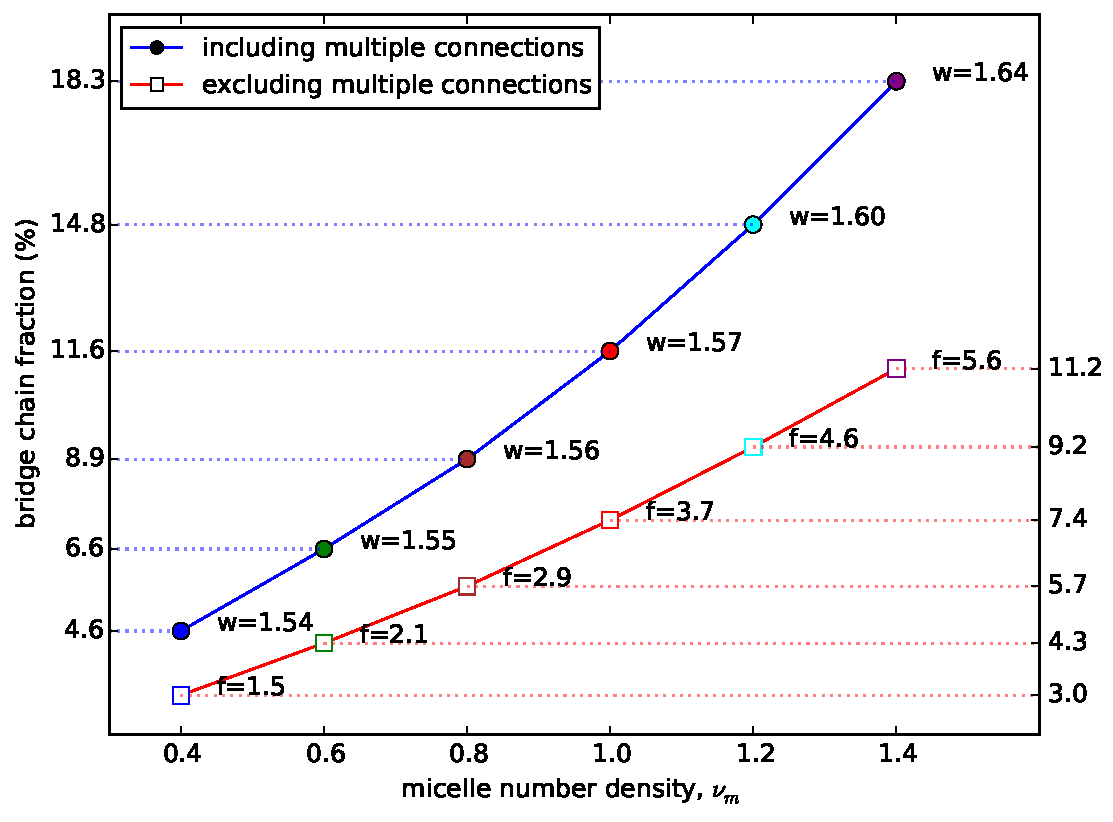
\includegraphics[height=0.7\textheight]{figures/bridge_chain_fraction_SUPOLEN_Leeds.pdf}
%   \caption{Fraction}
% \end{figure}
% \end{frame}

% \begin{frame}
% \frametitle{Stress Autocorrelation}
% \begin{figure}
%   \centering
%   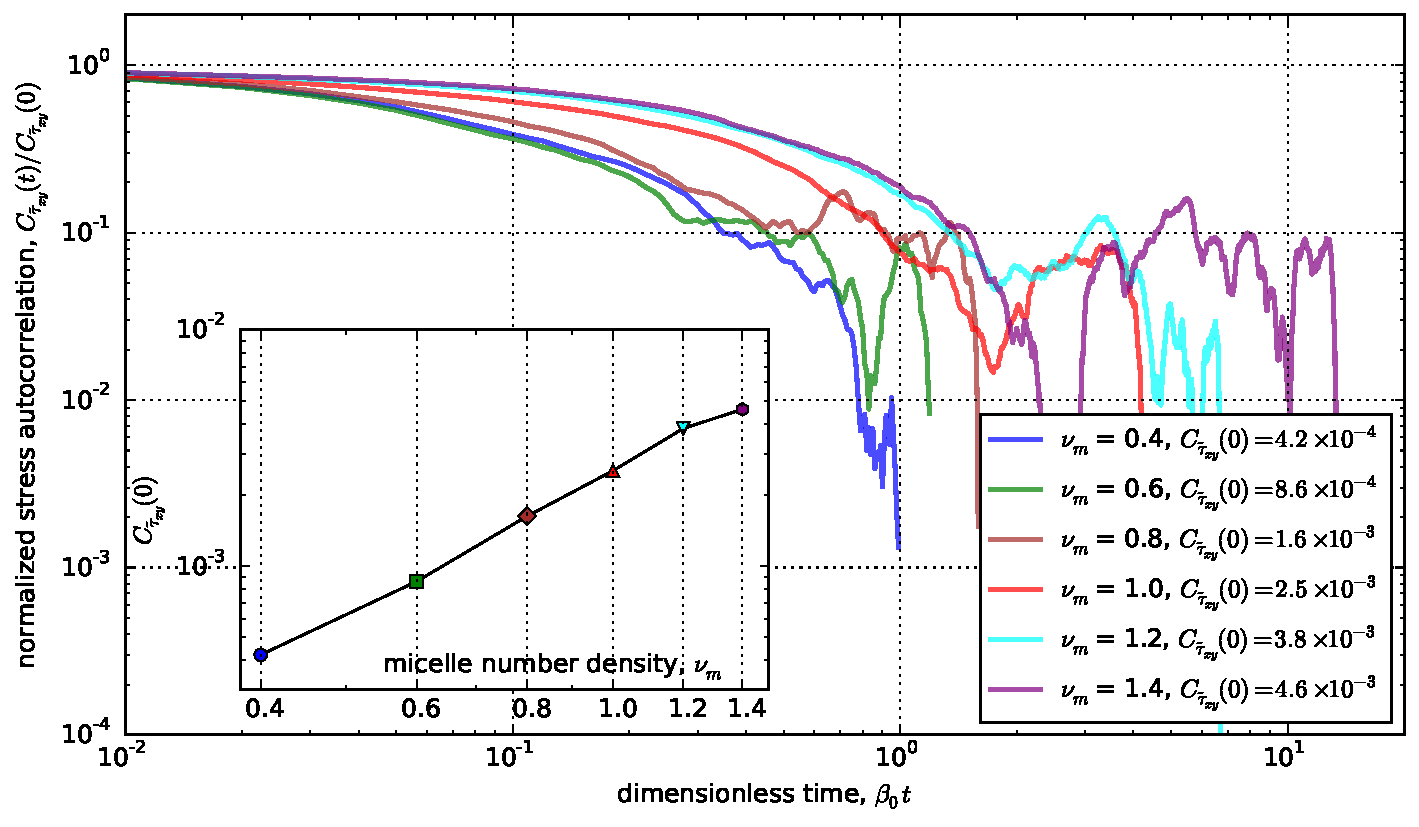
\includegraphics[height=0.7\textheight]{figures/ACF_refined_ICR_abstract_normalized.pdf}
%   \caption{Stress autocorrelation}
% \end{figure}
% \end{frame}

% \begin{frame}
% \frametitle{Mean Square Displacement}
% \end{frame}

% \begin{frame}
% \frametitle{Scaling Laws}

% \end{frame}

% \section{Conclusions}
% \begin{frame}
% \frametitle{Conclusions and Remarks}
% \end{frame}

% % \section{References}
% \begin{frame}[allowframebreaks]
%   \frametitle{Bibliography}
%   \printbibliography[nottype=url]
% \end{frame}

% \end{document}

% % \section{Overview}
% % \begin{frame}
% % \frametitle{Models for Transient Networks System \hfill[Crete]}
% % \begin{block}{Telechelic association system \parencite{Vaccaro:2000}}
% %   Evolution for attachment and detachment probability are represented by
% %   \begin{small}\begin{align}
% %     \frac{\partial }{\partial t}\Psi_{A} &= -\frac{\partial}{\partial \mathbf{R}}\cdot \mathbf{V}_{A} - \beta \Psi_A + \alpha \Psi_D;\\
% %     \frac{\partial }{\partial t}\Psi_{D} &= -\frac{\partial}{\partial \mathbf{R}}\cdot \mathbf{V}_{D} + \beta \Psi_A - \alpha \Psi_D,
% %     \end{align}\end{small}
% %   where $\alpha$ and $\beta$ are kinetic functions.
% %   % where $\alpha$ and $\beta$ are kinetic functions related to association and dissociation.
% % \end{block}
% % \centering\begin{small}\begin{tabular}{|c|c|c|}\hline
% %       Association($\alpha$) & Dissociation($\beta$) & \multicolumn{1}{c|}{Ref. \parencite{Tripathi:2006}}\\ \hline
% %       $1/\tau_E$ & $1/\tau_E$ & \small\textcite{Green:1946} \\ \hline
% %       $c_1\tau_E$ & $\exp(c_2R)/\tau_E$ & \small\textcite{Tanaka:1992_a, Tanaka:1992_b, Tanaka:1992_c} \\ \hline
% %       $(c_1 R/R_0)/\tau_E$ & $2/\tau_E$ & \small\textcite{VandenBrule:1995}\\ \hline
% %       $ (c_1 + c_2R/R_0)/\tau_E$ & $f/\tau_E$ & \small\textcite{Vaccaro:2000} \\ \hline
% %     \end{tabular}\end{small}
% % \end{frame}

% % %% \begin{frame}
% % %%   \frametitle{Simulation for Transient Networks System\hfill[Geleen]}
% % %%   \begin{block}{Coarse-Grained Models}
% % %%     \begin{itemize}
% % %%     \item \textcite{Koga:2005kz}: introduce individual sticky bead
% % %%     \item \textcite{Hoy:2009}: stochastic decision for association/dissociation
% % %%     \item \textcite{Li:2010bm}: control long-range interaction for donor and acceptor beads
% % %% % Using attractive bead \parencite{Koga:2005kz, Li:2010bm}
% % %% %     \item Using stochastic decision for associative bond \parencite{Hoy:2009}
% % %%     \end{itemize}
% % %%   \end{block}
% % %%   \begin{block}{Atomistic Molecular Dynamics}
% % %%     \begin{itemize}
% % %%     \item Association/dissociation mechanics is naturally builted-in based for given force field
% % %%     \item Time and length scales are restricted 
% % %%     \end{itemize}
% % %%   \end{block}
% % %% \end{frame}

% % \begin{frame}
% %   \frametitle{Atomistic Molecular Dynamics for Oligomer \hfill[Geleen]}
% %   \begin{block}{Without association: Flow induced friction reduction}
% %     \begin{itemize}
% %     \item Non-equilibrium MD (NEMD) simulation: steady shear flow with high flow rate ($\dot{\gamma} \geq \tau_R^{-1}$)
% %     \item Measure mobility($\mathbf{M}$), friction($\boldsymbol{\zeta}$), and diffusivity($\mathbf{D}$)
% %     \item Chemical dependency for friction reduction: Oligomer type PS, PMMA, PnBA
% %     \end{itemize}
% %   \end{block}
% %   \begin{block}{With association: Flow effects to the kinetic functions}
% %     \begin{itemize}
% %     \item Introduce sticky group for oligomer using TraPPE-UA force field
% %     \item Observe time scales for associative system and tuning using temperature controls
% %     \item Development the method to measure the kinetics
% %     \end{itemize}
% %   \end{block}
% % \end{frame}

% % \section{Methodology}

% % \begin{frame}
% %   \frametitle{Generating Initial Box for Oligomer}
% %   \begin{minipage}{0.6\textwidth}
% %   \begin{enumerate}
% %   \item Set the system and building molecules: SMILES string $\Rightarrow$ 3d structure
% %   \item Developing force fields based on TraPPE-UA force field
% %     \begin{itemize}
% %     \item Tree data structure for connected atoms
% %     \item Generating all connections for the force field using pre-order tree traversal method
% %     \item Generating all types for non-bonding potential
% %     \end{itemize}
% %   \item Equilibration
% %   \item Optimization computation efficiency
% %   \end{enumerate}
% %   \end{minipage}
% %   \begin{minipage}{0.38\textwidth}
% %     \begin{figure}
% %       \centering
% %       \includegraphics[width=\textwidth]{figures/preorder_tree.pdf}
% %       \caption{\small{Schematic diagram for pre-order travel for tree structure.}}
% %     \end{figure}
% %   \end{minipage}
% % \end{frame}

% % \begin{frame}
% %   \frametitle{TraPPE-UA force fields for PMMA and PnBA}
% %   \begin{block}{Bonded interactions}
% %     \begin{enumerate}
% %     \item Rigid bonding potential: $u_{12}(r) = l_0$
% %     \item Simple harmonic angle potential: $u_{13}(\theta) = \frac{k_\theta}{2}\left(\theta-\theta_0\right)^2$
% %     \item Dihedral potential: $V_n(\phi)=k_{\phi}(1+\cos(n\phi-\phi_s))$
% %     \end{enumerate}
% %   \end{block}
% %   \begin{block}{Non-bonded interaction}
% %     \begin{enumerate}
% %     \item Lennard-Jones 6-12 potentials with long-range correction
% %     \item Coulomb potential for electrostatic using Particle-Mesh Ewald Sum (PME)
% %     \end{enumerate}
% %   \end{block}
% %   All the detail parameters are extracted by \textcite{Maerzke:2009, Kamath:2006, Stubbs:2004, Sokkalingam:2009, Ferrando:2012}.
% % \end{frame}


% % \begin{frame}
% %   \frametitle{Diffusivity and Mean Square Displacement}
% %   \vspace{-0.2in}
% %   \begin{figure}
% %     \hspace{-0.5in}
% %     \begin{minipage}[b]{0.75\textwidth}
% %       \centering
% %       \includegraphics[width=\textwidth]{figures/msd_compare_AHT_SHT_REF.pdf}
% %     \end{minipage}
% %     \hspace{-0.3in}
% %     \begin{minipage}[b]{0.3\textwidth}
% %       \caption{\small{Mean-square displacement for PMMA decamer and comparison with \textcite{Chen:2008ec}. The symbol is for reference data, solid line represent NVT simulation with typical PMMA density, and dashed lines are NPT simulationa.}}
% %     \end{minipage}
% %   \end{figure}
% % \end{frame}


% % \begin{frame}
% %   \frametitle{Time Scales and Computation Limitations}
% %   \vspace{-0.1in}
% %   \begin{block}{Correlation function for end-to-end vector}
% %     Let $\mathbf{P}(t)$ is end-to-end vector for a molecule, the correlation is given by
% %     \begin{equation}
% %       Corr[\mathbf{P}, \mathbf{P}](t) = \langle \mathbf{P}(\xi)\cdot\mathbf{P}(\xi + t)\rangle_{\xi} \propto \exp\left(-\frac{t}{\tau_R}\right)\textrm{ for }t \geq \tau_R,
% %     \end{equation}
% %     where $\tau_R$ is the longest characteristic time for the end-to-end vector.
% %   \end{block}
% %   \vspace{-0.1in}
% %   \begin{figure}
% %     \begin{minipage}[b]{0.50\textwidth}
% %       \centering
% %       \includegraphics[width=0.83\textwidth]{figures/acf_500_600.pdf}
% %     \end{minipage}
% %     \begin{minipage}[b]{0.40\textwidth}
% %       \caption{\small{Results of autocorrelation function for PMMA decamer at 500K and 600K. The plot represents almost single exponential decay which make simple to calculation characteristic time.}}
% %     \end{minipage}
% %   \end{figure}
% % \end{frame}


% % \begin{frame}
% %   \frametitle{Constant Pulling for Mobility and Friction Tensors}
% %   \begin{block}{Mobility Tensor}
% %     Because of isotropic nature of the system, the long-time average for velocity and force exerted on the pulled molecule can be presented by 
% %     \begin{small}\begin{equation}
% %       \langle \mathbf{v}\rangle_{t, p} = \mathbf{M}\cdot\langle\mathbf{f}\rangle,\label{eq:mobility}
% %     \end{equation}\end{small}
% %     where $\mathbf{M}$ is mobility tensor, $\mathbf{f}$ is pulling constant, and $t$ and $p$ denote the average taking over the time and pulled molecules.
% %   \end{block}
% %   In equilibrium, when pulling force is appropriately choose, the diffusion coefficient, $D_{eq}$, and mobility, $M_{eq}$, can be connected by Einstein-Stokes relation:
% %   \small{\begin{equation}
% %     D_{eq} = k_BT M_{eq},\label{eq:einstein_stokes}.
% %   \end{equation}}

% % \end{frame}

% % \begin{frame}
% %   \frametitle{Constant Pulling for Mobility and Friction Tensors (cont.)}
% %   \begin{figure}
% %     \centering
% %     \includegraphics[width=0.49\textwidth]{figures/X_components_for_pulled_molecule.pdf}
% %     \includegraphics[width=0.49\textwidth]{figures/diffusivity_compare.pdf}
% %     \caption{\small{(left) X trajectory for pulled molecules with different pulling force. (right) Calculated diffusion coefficient in equilibrium from average mean-square-displacement for unpulled molecule (blue symbol) and converted diffusion coefficient using Einstein-Stokes relation (red symbol).}}
% %   \end{figure}
% % \end{frame}




% % \begin{frame}
% %   \frametitle{Boundary Driven Algorithm for Steady Shear Flow}
% %   \vspace{-0.1in}
% %   \begin{figure}
% %     \begin{minipage}[b]{0.5\textwidth}
% %       \centering
% %       \includegraphics[width=0.8\textwidth]{figures/boundary_driven_shear.png}
% %     \end{minipage}
% %     \begin{minipage}[b]{0.45\textwidth}
% %       \caption{\small{Schematic diagram to depict boundary driven shear flow so-called Lee-Edwards sliding bricks. This is valid for time independent flow.}}
% %     \end{minipage}
% %   \end{figure}
% %   \vspace{-0.1in}
% %   The Lagrangian coordinate for the trajectory is results of following correction:
% %     \begin{equation}
% %       X_{CM}^{\ast(k)}(t) = X_{CM}^{(t)}(t) - \dot{\gamma}\int_0^t Y_{CM}^{(k)}(t')dt',
% %     \end{equation}
% %     where $X_{CM}$, $Y_{CM}$, and $Z_{CM}$ are given xyz components for trajectory.
    
% % \end{frame}

% % \section{Conjecture}
% % \begin{frame}
% %   \frametitle{Interpretation of Time Scales}
% %   \begin{minipage}[b]{0.5\textwidth}
% %     \begin{block}{Tuning temperature for PMMA}
% %       \begin{itemize}
% %       \item Tg for PMMA around 380K (atatic)
% %       \item Density for PMMA is around 1.066 (g/cm$^3$)
% %       \item 100 decamer (PMMA):
% %         \begin{itemize}
% %         \item 1-2 ns for 1 hour
% %         \item For $\tau_R\approx 10$(ns), 200-300ns\\ $\Rightarrow$ 10-20 days
% %         \end{itemize}
% %       \item From 500K to 600K:
% %         \begin{itemize}
% %         \item density: 1.03 $\rightarrow$ 0.96 (g/cm$^3$)
% %         \item $\tau_R$: 8.8 $\rightarrow$ 1.2 (ns)
% %         \end{itemize}
% %       \end{itemize}
% %     \end{block}
% %   \end{minipage}
% %   \hspace{0.1in}
% %   \begin{minipage}[b]{0.4\textwidth}
% %     \begin{figure}
% %       \includegraphics[width=\textwidth]{figures/shift_factor_anal_PMMA.pdf}
% %       \caption{\small{Interpretation of time scales and density profiles with respect to temperature. The expected scheme is followed typical PMMA data.}}
% %     \end{figure}
% %   \end{minipage}
% % \end{frame}

% % \begin{frame}
% %   \frametitle{Interpretation of Time Scales for PnBA with Association}
% %   \vspace{-0.1in}
% %   \begin{block}{PnBA + Association}
% %     \begin{itemize}
% %     \item At 373K, time scale is around 10ns (Tg for PnBA is around 200K)
% %     \item Longer relaxation time for associative system
% %     \item Different temperature dependence for association and oligomer dynamics
% %     \end{itemize}
% %   \end{block}
% %   \begin{figure}
% %   \begin{minipage}{0.7\textwidth}
% %     \includegraphics[width=\textwidth]{figures/pba_association.png}
% %   \end{minipage}
% %   \begin{minipage}{0.25\textwidth}
% %     \caption{PnBA with hydrogen bonding side group with different bonding strength \parencite{Lewis:2014fs}.}
% %   \end{minipage}
% %   \end{figure}
% % \end{frame}

% % \section{Conclusions}
% % \begin{frame}
% %   \frametitle{Summary and Future Works}
% %   \begin{enumerate}
% %   \item The research object is effects of flow to the kinetic functions
% %   \item For the simplicity of implementation for differemt material systems, atomistic MD simulation is selcted 
% %   \item For steady shear flow, the sliding bricks concept make easy to implement for PBC
% %   \item For computational limitation, the longest relaxation time for end-to-end vector should be around 10 ns
% %   \item Effects of temperature to the oligomer dynamics and association/dissociation kinetics has different role that make difficulty to tuning time scales of the system
% %   \item When objective system has outside of processing time scales, coarse-grained simulation is under the consideration to perform
% %   \end{enumerate}
% % \end{frame}


